% Lecture Template for ME3050-001-002-Tristan Hill - Spring 2020
% Dynamics Modeling and Controls
% Time Response - Lecture 3

% I am finally converting my stuff to BEAMER

% Document settings

%\documentclass{beamer}                  % for presentation ?
\documentclass[handout]{beamer}  % for handout ?
\usepackage{beamerthemesplit}
\usepackage{amsmath}
\usepackage{listings}
\usepackage{multicol}
\usepackage{framed}
\usepackage{amssymb}


\lstdefinestyle{myCustomMatlabStyle}{
  language=Matlab,
  numbers=left,
  stepnumber=1,
  numbersep=10pt,
  tabsize=4,
  showspaces=false,
  showstringspaces=false
}
\lstset{basicstyle=\ttfamily\tiny,style=myCustomMatlabStyle}
%lstset{language=MATLAB,basicstyle=\ttfamily\small,showstringspaces=false}



\beamertemplateballitem

\definecolor{TTUpurple}{rgb}{0.3098, 0.1607, 0.5176} % TTU Purple (primary)
\definecolor{TTUgold}{rgb}{1.0000, 0.8666, 0.0000} % TTU Gold (primary)

\setbeamercolor{palette primary}{bg=TTUpurple,fg=TTUgold}
\setbeamercolor{palette secondary}{bg=black,fg=TTUgold}
\setbeamercolor{palette tertiary}{bg=black,fg=TTUpurple}
\setbeamercolor{palette quaternary}{bg=TTUgold,fg=black}
\setbeamercolor{structure}{fg=TTUpurple} % itemize, enumerate, etc
\setbeamercolor{section in toc}{fg=TTUpurple} % TOC sections

%\DeclareSymbolFont{bbold}{U}{bbold}{m}{n}
%\DeclareSymbolFontAlphabet{\mathbbold}{bbold}

%\newcommand{\bbfamily}{\fontencoding{U}\fontfamily{bbold}\selectfont}
%\DeclareMathAlphabet{\mathbbold}{U}{bbold}{m}{n}

%\usefonttheme{professionalfonts}

\newcommand{\vspccc}{\vspace{6mm}\\} % large vertical space
\newcommand{\vspcc}{\vspace{4mm}\\}   % medium vertical space
\newcommand{\vspc}{\vspace{2mm}\\}     % small vertical space

\newcommand{\hspcccc}{\hspace{10mm}} % large horizontal space
\newcommand{\hspccc}{\hspace{6mm}} % large horizontal space
\newcommand{\hspcc}{\hspace{4mm}}   % medium horizontal space
\newcommand{\hspc}{\hspace{2mm}}     % small horizontal space


\newcommand{\LT}{\mathcal{L}} % lagrangian

\newcommand{\LNUM}{1} %Lecture number 1

\newcommand{\secondtitle}{Frequency Response of First Order Systems}% second line of the title of this presentation , aka the topic of this lecture

\title{Frequency Response - Lecture \LNUM}
\author{ME3050 - Dynamics Modeling and Controls} % original formatting from Mike Renfro, September 21, 2004

\date{April  19, 2020}

\begin{document}

\lstset{language=MATLAB,basicstyle=\ttfamily\small,showstringspaces=false}

% Title page1 
\frame{\titlepage \center\textbf{\secondtitle}\vspcc}


% Section 0: Outline
\frame{

\large \textbf{Lecture \LNUM - \secondtitle} \vspc

 \begin{itemize}

	\item Introduction to Chapter 9\vspc % Section 1: The Step Input

	\item Review Complex Numbers\vspc        % Section 2
	
	\item Frequency Response of First Order Systems\vspc %Section 3

	\item Graph of System Response\vspace{2mm} % Section 4

\end{itemize}

}


%Section 1: Introduction to Chapter 9
\section{Introduction to Chapter 9}

\subsection{Harmonic Input Function}
\frame{
\frametitle{Harmonic Input Function}

\small 
The term {\bf frequency response} is used to describe a system's response to a periodic input. Frequency response analysis focuses on a system's response to {\it harmonic} input such as sines and cosines. The input (forcing) function is written below.\vspcc


\begin{framed}
\scalebox{1.25}{$f(t)=Asin\left(\omega t\right)$}\vspccc

\renewcommand{\arraystretch}{1.5}
\begin{tabular}{ccc}
Amplitude of the Input, & \scalebox{1}{$A$} & \scalebox{1}{$ (N)$} \\
Frequency of Input, &\scalebox{1}{$\omega$} &  \scalebox{1}{$(\frac{rad}{s})$}\\
\end{tabular}
\end{framed}

}


\subsection{Why Study Frequency Response?}
\frame{
\frametitle{Why Study Frequency Response?}
\small
 Why do we care about the way a system responds to harmonic excitation? Why is {\bf frequency analysis} important? \\
\begin{itemize}
\item
\item
\item
\end{itemize}

\vspace{3mm}What causes {\bf harmonic} (or sinusoidal) excitation in the real world? \\

\begin{itemize}
\item
\item
\item
\end{itemize}

}

\subsection{Frequency Response and the Transfer Function}
\frame{
\frametitle{Frequency Response and the Transfer Function}

A linear, time-invariant (LTI) system has a {\bf transfer function} $T(s)$ that describes the {\bf input-output} relationship of the system. Under sinusoidal excitation (input) with frequency $\omega$ if the system is stable the transient affects in the response (output) will eventually disappear leaving the {\bf steady state sinusoidal response} of the same frequency as the input but with a phase shift w.r.t. the input.

}

% section 2: Review Complex Numbers

\section{Review Complex Numbers}

\subsection{The Complex Plane}
\frame{
\frametitle{The Complex Plane}

In an underdamped system the roots of the characteristic polynomial are complex. Before we proceed we need to review some rules of arithmetic and complex numbers. \vspc

\begin{multicols}{2}
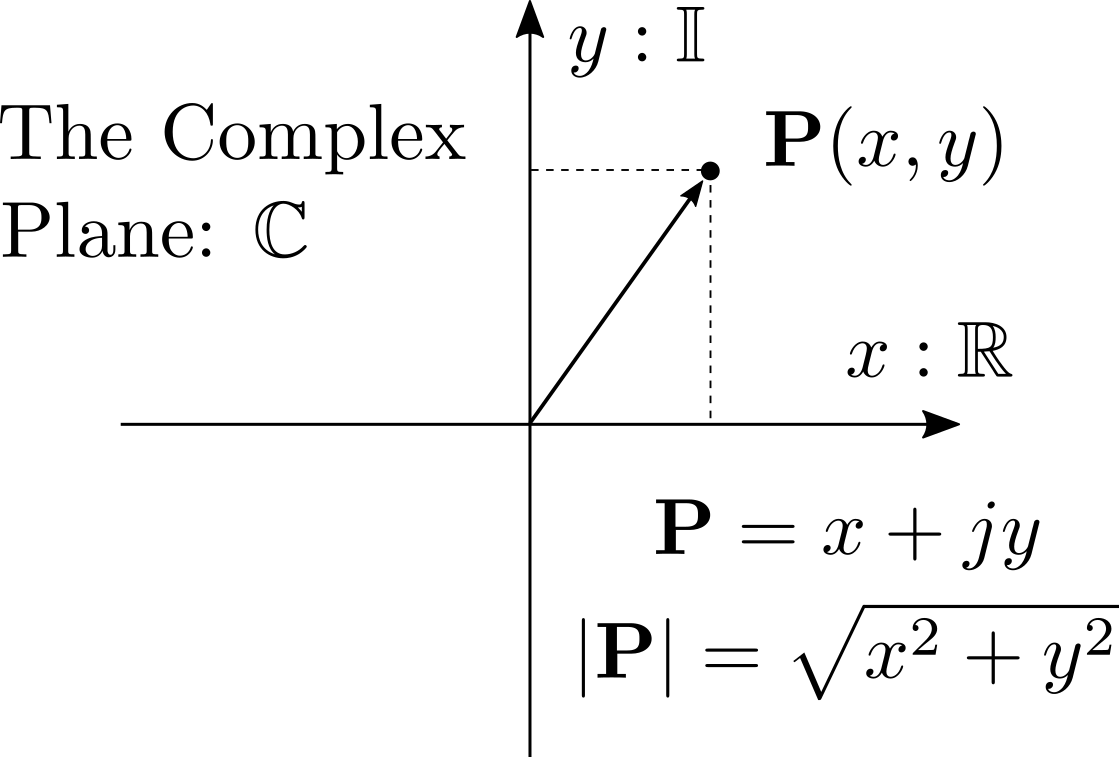
\includegraphics[scale=0.175]{lecture1_fig1.png}

\small
\hspccc Cartesian Representation:\vspc\hspccc\scalebox{.8}{$\mathbf{P}=x+jy$}\vspc
\hspccc Polar Representation:\vspc\hspccc\scalebox{.8}{$\mathbf{P}=|\mathbf{P}|\angle\theta$}\vspc
\hspccc Exponential Representation:\vspc\hspccc\scalebox{.8}{$\mathbf{P}=|\mathbf{P}|e^{j\theta}=|\mathbf{P}|\left(cos\theta+jsin\theta\right)$}\vspc
\end{multicols}

}



\subsection{Complex Number Algebra}
\frame{
\frametitle{Complex Number Algebra}
 
 Consider two points $\mathbf{P_1}$ and $\mathbf{P_2}$ on the complex plane. \vspc
 
 \scalebox{1}{$\mathbf{P_1}=x_1+jy_1$\hspc and \hspc$\mathbf{P_2}=x_2+jy_2$} \vspccc
\renewcommand{\arraystretch}{1.75}
 \begin{tabular}{cc}
 Addition:& \scalebox{1}{$\mathbf{P_1}+\mathbf{P_2}=(x_1+x_2)+j(y_1+y_2)$}\\
 Multiplication:& \scalebox{1}{$\mathbf{P_1P_2}=|\mathbf{P_1P_2}|\angle\left(\theta_1+\theta_2\right)$}\\
 Division:&\scalebox{1}{$\frac{\mathbf{P_1}}{\mathbf{P_2}}=(x_1+x_2)+j(y_1+y_2)$}\\
\end{tabular}

}


% section 3: Frequency Response of First Order Systems

\section{Frequency Response of First Order Systems}

\subsection{Frequency Response of First Order Systems}
\frame{
\frametitle{Frequency Response of First Order Systems}

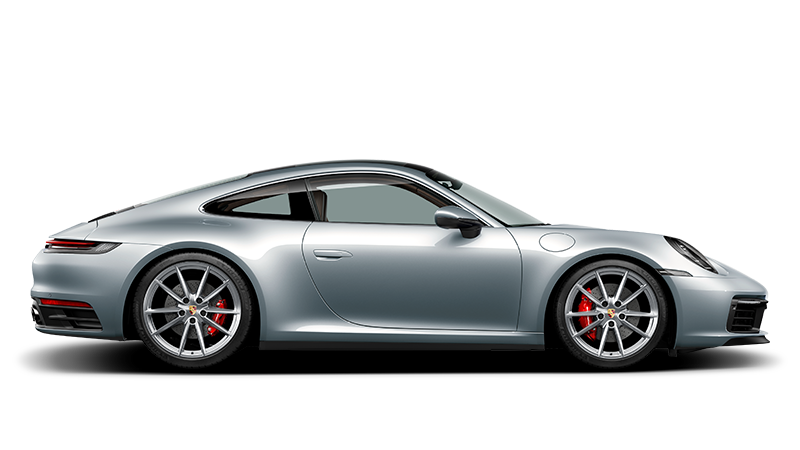
\includegraphics[scale=.15]{porsche.png}

Consider our $1^{\underline{st}}$ order mass damper system. \vspc

\scalebox{1}{$m\dot{v}+cv=f(t)$} \hspcc with a {\bf time constant} \scalebox{1}{$\tau=\frac{m}{c}$} \vspcc

The system is commonly re-written as shown below. \vspc

\scalebox{1}{$m\dot{v}+cv=f(t)\hspc\rightarrow\hspc\tau\dot{y}+y=f(t)$} \vspc

}

\subsection{Obtain the Transfer Function}
\frame{
\frametitle{Obtain the Transfer Function}

\small

\scalebox{1}{$\tau\dot{y}+y=f(t)$} \vspcc

Take the Laplace transform of the ODE. \vspcc

\scalebox{1}{$\LT\{\tau\dot{y}+y\}=\LT\{f(t)\}$} \vspcc

\scalebox{1}{$\tau\left(sY(s)+y_0)\right)+Y(s)=F(s)$}\hspccc The initial conditions are zero. \vspcc

\begin{framed}
\scalebox{1}{$T(s)=\frac{Y(s)}{F(s)}=\frac{1}{\tau s+1}$}\hspccc First Order Transfer Function
\end{framed}

This considers a {\it generalized} input function $f(t)$ and zero ICs.
}

\subsection{Sinusoidal Input Function}
\frame{
\frametitle{Sinusoidal Input Function}

\small

Our model is now excited by a sinusoidal input (forcing) function. \vspc

\scalebox{1}{$\tau\dot{y}+y=f(t)=Asin\left(\omega t\right)$} \vspc

Take the Laplace Transform. Then, solve for $Y(s)$ and expand.\vspc

\scalebox{1}{$\tau sY(s)+Y(s)=\frac{A\omega}{s^2+\omega^2}$}  \vspc

\scalebox{1}{$Y(s)=\frac{A\omega}{\left(s^2+\omega^2\right)\left(\tau s+1\right)}=\frac{C_1}{\tau s+1}+\frac{C_2s}{\left(s^2+\omega^2\right)}+\frac{C_3\omega}{\left(s^2+\omega^2\right)}$} \vspc

Now solve for the coefficients.\vspc

\scalebox{1}{$C_1=\frac{A\omega\tau^2}{1+\omega^2\tau^2}\hspccc,\hspc C_2=\frac{-A\omega\tau}{1+\omega^2\tau^2}\hspccc,\hspc C_3=\frac{A}{1+\omega^2\tau^2}$} \vspc

Substituting and take the inverse Laplace transform. \vspc
\scalebox{1}{$y(t)=\frac{A\omega\tau}{1+\omega^2\tau^2}\big( e^{\frac{-t}{\tau}}-cos\omega t+\frac{1}{\omega\tau}sin\omega t\big) $}

}

\subsection{Steady State Time Response}
\frame{
\frametitle{Steady State Time Response}

\small
\scalebox{1}{$y(t)=\frac{A\omega\tau}{1+\omega^2\tau^2}\big( e^{\frac{-t}{\tau}}-cos\omega t+\frac{1}{\omega\tau}sin\omega t\big) $} \vspcc
After some amount of time passes, the transient term will disappear leaving just the sinusoidal terms. \vspcc

\scalebox{1}{$y(t)=\frac{A}{1+\omega^2\tau^2}\big(sin\omega t - \omega\tau cos\omega t\big) $} \vspccc
This is re-written as a single sinusoidal term with a phase shift. \vspc

\begin{framed}
Steady State Frequency Response of First Order System\vspc
\scalebox{1}{$y(t)=\frac{A}{\sqrt{1+\omega^2\tau^2}}sin\left(\omega t+\phi\right) \hspccc,\hspc \phi=-tan^{-1}\omega\tau$}
\end{framed}

}

\subsection{Amplitude Ratio}
\frame{
\frametitle{Amplitude Ratio}

\small

\scalebox{1}{$y(t)=\frac{A}{\sqrt{1+\omega^2\tau^2}}sin\left(\omega t+\phi\right) \hspccc,\hspc \phi=-tan^{-1}\omega\tau$} \vspccc

Notice that the system responds at the same frequency as the input but with a different amplitude and a phase shift. The ratio of the response amplitude to the input amplitude is called the {\bf amplitude ratio, M}. \vspc

\scalebox{1}{$M=\frac{\frac{A}{\sqrt{1+\omega^2\tau^2}}}{A}=\frac{1}{\sqrt{1+\omega^2\tau^2}}$} \vspc

Fortunately we can find the {\bf amplitude ratio} and {\bf phase shift} directly from the transfer function. Recall the transfer function we derived. \vspc

\scalebox{1}{$T(s)=\frac{1}{\tau s+1}$}\hspccc let \scalebox{1}{$s=j\omega\hspccc\implies\hspccc T(j\omega)=\frac{1}{\tau j\omega+1}$} \vspc

\scalebox{1}{$|T(j\omega)|=\frac{|1|}{|\tau j\omega+1|}=\frac{1}{\sqrt{\left(\tau\omega\right)^2+1^2}}=\frac{1}{\sqrt{1+\tau^2\omega^2}}$} \hspccc \hspccc Look familiar? \vspc 

}

\subsection{Amplitude Ratio and Phase Angle}
\frame{
\frametitle{Amplitude Ratio and Phase Angle}

\small

\scalebox{1}{$|T(j\omega)|=\frac{1}{\sqrt{1+\tau^2\omega^2}}=M$}\vspc

\scalebox{1}{$\angle T\left(j\omega\right)=\angle 1-\angle\left(1+j\omega\tau\right)=tan^{-1}\left(\frac{0}{1}\right)-tan^{-1}\left(\frac{\omega\tau}{1}\right)=-tan^{-1}\left(\omega\tau\right)=\phi$}\vspcc

Substitute $s=j\omega$ into the transfer function and solve for the magnitude and phase angle of this complex number which represent the magnitude ratio and phase shift. \vspc

Therefore the steady state response is written as follows.  \vspc

\scalebox{1}{$y_{ss}\left(t\right)=A|T\left(j\omega\right)|sin\left(\omega t+\angle T\left(j\omega\right)\right)=MAsin\left(\omega t+\phi\right)$}\vspcc

Wasn't that fun? Can you believe we used to do that on the board?!?! \vspc
}

\subsection{Graph of Frequency Response}
\frame{
\frametitle{Graph of Frequency Response}

\small

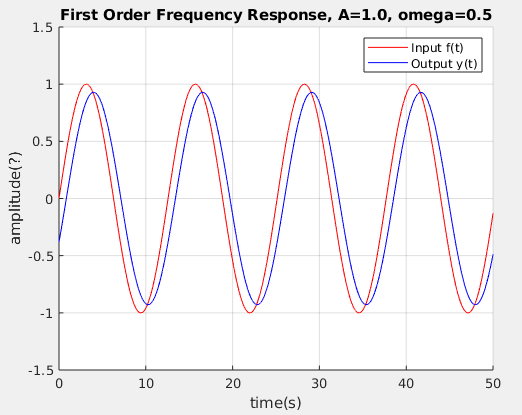
\includegraphics[scale=.275]{lecture1_fig6.png} \hspc 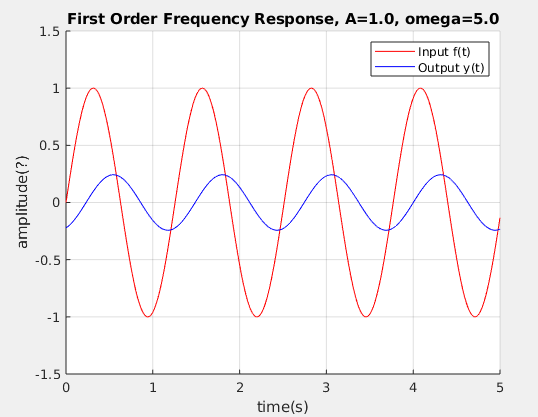
\includegraphics[scale=.275]{lecture1_fig5.png}  \vspc

What determines the amplitude of the system response? \vspc

}


\subsection{MATLAB code}

\frame[containsverbatim]{
\frametitle{MATLAB code}

\begin{lstlisting}
% ME3050 - Spring 2020 Tennessee Technological Univ.
clear variables;clc;close all

% define the system parameters
m=20;c=25;
tau=m/c;

% define the amplitude input frequency and
A=1;omega=1/2;

% calculate the magnitude ratio
M=1/sqrt(1+omega^2*tau^2);
phi=-tan(omega*tau);


\end{lstlisting}

}
\frame[containsverbatim]{
\frametitle{MATLAB code}

\begin{lstlisting}
%consider a range of time values
dt=0.01;tstop=50;
time=0:dt:tstop;
 
%calculate the input and response curves
fin=A*sin(omega*time);
yout=M*A*sin(omega*time+phi);

% show the results in a figure
figure(1);hold on
plot(time,fin,'r')
plot(time,yout,'b')

\end{lstlisting}

}
% references is not a section for now, for looks and it would be a waste of space
\frame{

\frametitle{References}

\begin{itemize}
	\item System Dynamics, Palm III, Third Edition - Chapter 9 - System Response in the Frequency Domain
\end{itemize}

}

\end{document}









 